\label{sec:delta}

\begin{figure}[!htbp]
\centering
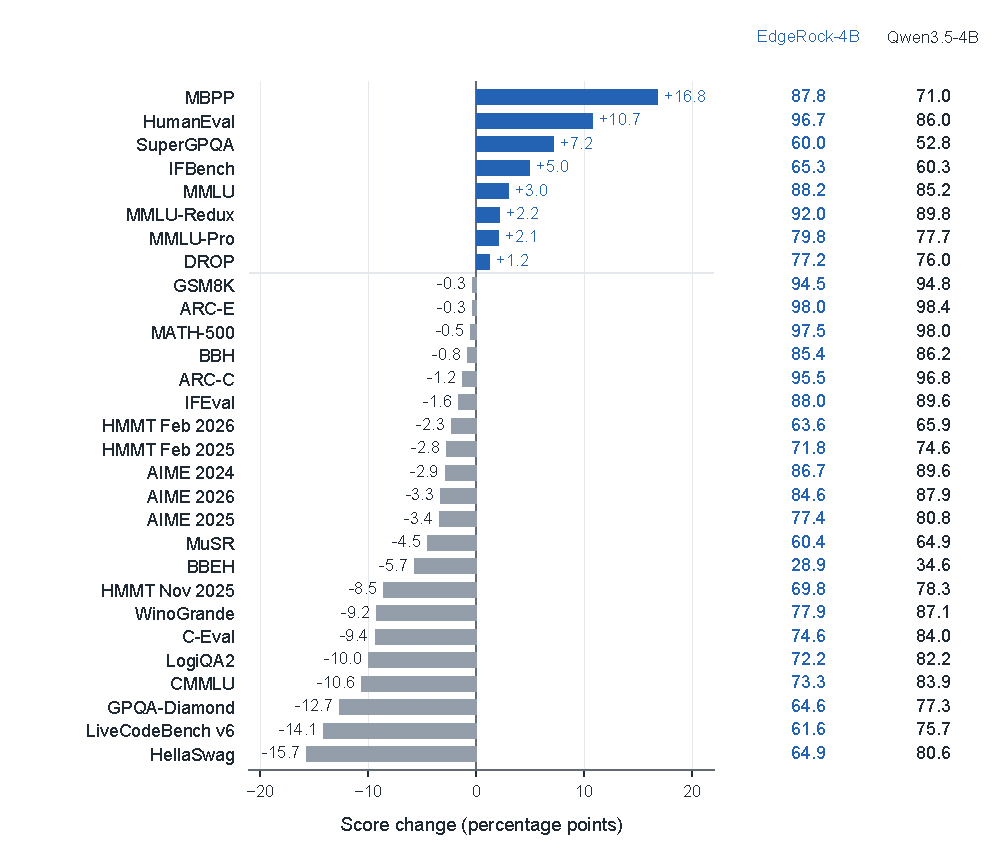
\includegraphics[width=\linewidth]{backbone_delta.pdf}
\caption{\textbf{Capability after conversion.} Bars report EdgeRock-4B minus its Qwen3.5-4B source backbone in percentage points, ordered from largest to smallest. Blue highlights the eight benchmark gains; aligned columns give absolute scores (\%).}
\label{fig:delta}
\end{figure}

\subsection{In the range of compact models with growing memory}
\label{sec:peer-capability}
Against compact models whose histories grow, EdgeRock-4B reasons in the same range. On AIME 2024--2026, its 82.9\% lies between Granite4.2-3B (82.2\%) and Qwen3.5-4B (86.1\%), with MiniCPM5-2B at 87.8\%, and well above Nemotron-3-Nano-4B (57.1\%), LFM2.5-2.6B (56.2\%), Gemma4-E4B (40.1\%), and Phi-4-mini-reasoning (38.9\%) (Table~\ref{tab:peer-capability}; Appendix~\ref{app:growing-results}). EdgeRock-4B scores higher than MiniCPM5-2B on MMLU-Pro and SuperGPQA, which test knowledge-intensive reasoning (Table~\ref{tab:peer-capability}).

EdgeRock-4B also leads LFM2.5-2.6B on \textbf{28 of 29 benchmarks} (Appendix~\ref{app:growing-results}).

\PeerCapabilityResults

\Needspace{17\baselineskip}
\subsection{Vision retained at constant memory}
\label{sec:vision}

EdgeRock-4B extends its constant-memory design to text-and-image reasoning. Across six visual benchmarks covering perception, chart and diagram understanding, and visual question answering, it reaches an \textbf{84.9\%} equal-weight mean answer-level accuracy, compared with 89.1\% for Qwen3.5-4B, retaining 95.3\% (Table~\ref{tab:visual-results}).

\begin{table}[!htbp]
\centering
\caption{Visual answer-level accuracy (\%), including MME. Retained gives EdgeRock-4B as a percentage of Qwen3.5-4B. Appendix~\ref{app:protocol} gives standard MME points.}
\label{tab:visual-results}
\begin{tabularx}{\linewidth}{@{}Yrrr@{}}
\toprule
Benchmark & EdgeRock-4B & Qwen3.5-4B & Retained (\%)\\
\midrule
MMBench EN~\cite{mmbench} & 88.3 & 90.1 & 98.0 \\
MMBench CN~\cite{mmbench} & 89.0 & 91.4 & 97.4 \\
POPE~\cite{pope} & 85.4 & 88.8 & 96.2 \\
MME~\cite{mme} & 83.0 & 86.8 & 95.6 \\
ChartQA~\cite{chartqa} & 83.9 & 90.3 & 92.9 \\
AI2D~\cite{ai2d} & 80.0 & 87.0 & 92.0 \\
\midrule
Equal-weight mean & 84.9 & 89.1 & 95.3 \\
\bottomrule
\end{tabularx}
\end{table}


\FloatBarrier
